\documentclass[a4paper,11pt]{article}
\usepackage[utf8]{inputenc}
\usepackage[paper=a4paper, hmargin=1.5cm, bottom=1.5cm, top=3.5cm]{geometry}
\usepackage[T1]{fontenc}
\usepackage[colorlinks=true, linkcolor=blue]{hyperref} %Links para el indice.
\usepackage{amsfonts}
\usepackage{verbatim}
\usepackage{listings}
\usepackage{caption}
\usepackage{subcaption}
\usepackage{graphicx}
\usepackage{wrapfig}
\usepackage[section]{placeins}
\usepackage{float}
%\usepackage{adjustbox}
\usepackage{amsmath}
\usepackage{blindtext}
\usepackage{sidecap}
\usepackage{color}

\captionsetup[subfigure]{labelformat=empty}

% \newcommand{\real}{\hbox{\bf R}}

\newcommand{\rto}{\textit{rto}}
\newcommand{\rtt}{\textit{rtt}}

\title{Conexiones}

\begin{document}

\maketitle

\begin{center}
	Universidad de Buenos Aires - Departamento de Computaci\'on - FCEN
\end{center}

\vspace{2cm}
Integrantes:

\begin{itemize}
	\item Gallardo, Guillermo L.U.: 32/10 \verb+gagdiez.c@gmail.com+
	\item Fixman, Martin L.U.: 391/11 \verb+martinfixman@gmail.com+
	\item Matayoshi, Leandro L.U.: 79/11 \verb+leandro.matayoshi@gmail.com+
	\item Szyrej, Alexander L.U.: 642/11 \verb+alexander.szyrej@gmail.com+

\end{itemize}

\newpage

\tableofcontents

\newpage

\section{Introducci\'on}
    
    Los protocolos confiables de transporte permiten al usuario abstraerse 
    de los problemas de transmisi\'on de la red, por ej, el protocolo TCP 
    nos permite enviar mensajes a traves de medios que pierden, desordenan
    y modifican paquetes. 
    
    El protocolo PTC es una implementaci\'on de la catedra, el mismo est\'a 
    basado en TCP, por lo tanto, intenta asegurar que los paquetes lleguen de un
    punto a otro utilizando diversos mecanismos como control de flujo, realizar
    la conexi\'on en etapas, mantener una ventana deslizante para enviar 
    y recibir paquetes, etc. 
        
    En este trabajo estudiaremos como se comporta PTC, poniendo especial 
    atenci\'on a la retransmisi\'on de paqutes. Para ello 
    primero emularemos escenarios donde existan delay y perdida
    de paquetes entre dos nodos comunicados. Luego, iremos modificando
    par\'ametros de la implementaci\'on para ver como ello afecta el reenvio 
    de paquetes. 


\section{M\'etodos}

    El protocolo PTC utiliza un sistema de \textit{acknowledge} para
    saber si un paquete fue recibido. En caso de no recibir un \textit{ack}
    para un  determinado paquete luego de un umbral de tiempo, procede a
    retransmitirlo. Dicho umbral, denominado \textit{rto} se va estimando
    a medida que se reconocen los paquetes enviados usando las
    siguientes funciones:

        $$RTTVAR = (1-\beta)RTTBAR + \beta |SRTT-RTT|$$
        $$SRTT = (1-\alpha)SRTT + \alpha RTT$$
        $$RTO = SRTT + max( 1, K * RTTVAR) $$

    Donde $K, \alpha, \beta \in \mathbb{Q}$, $RTT$ es el valor de
    \textit{rtt} calculado para el \'ultimo \textit{ack} recibido.
    En la implementaci\'on utilizada se inicializan los valores de la
    siguiente manera: $K = 4, \alpha={{1}\over{8}}$,
    $\beta={{1}\over{4}}$, $SRTT={RTT_0}$, $RTTVAR={{RTT}\over{2}}$.
    Siendo $RTT_0$ el primer \textit{rtt} calculado.

\subsection{Sistema}

	Tanto el cliente como el servidor est\'an simulados en el mismo sistema. La
	topolog\'ia de este sistema es similar a la de dos equipos, un cliente y un
	servidor, conectados mediante un link ethernet en la misma red o en
	diferentes redes pero con cierto nivel previsible de congesti\'on.

	Al protocolo PTC se le puede artificialmente poner un \emph{delay} ficticio,
	que simular\'ia tanto la distancia que hay entre en cliente y el servidor en
	la red simulada como el nivel de congesti\'on entre estos dos puntos.
  Por ejemplo, en los entornos reales (muy distintos al de nuestra experimentaci\'on),
  el delay incluye el tiempo en el que
  los paquetes permanecen en los buffers de cada router antes de ser forwardeados,
  el cual puede ser un factor a tener en cuenta para medir el nivel de congesti\'on
  de una red.
	Tambi\'en se tiran adrede los paquetes con una probabilidad $p$, simulando
	la perdida de paquetes que puede pasar en una red congestionada o con links
	erroneos.

	Dada la velocidad de procesamiento actual, sumado al procesamiento en
	paralelo, podemos asumir que el RTT real es el delay ficticio que generamos,
	dado que un tick simulado ronda el orden del mill\'on de tick reales.

	En lo que respecta a este TP, todas las conexiones son conexiones que usan
	el protocolo PTC.


\section{Desarrollo}

    En primera instancia se implementaron dos scripts en python que 
    actuan uno como cliente y otro como servidor.
    Luego, se modific\'o la implementaci\'on de PTC para poder simular
    delay y perdida de paquetes (el contexto de una red), adem\'as de transformar en par\'ametros
    a los valores $\alpha$ y $\beta$ para estudiar como se modifica el
    \rto{} en base a los mismos.  

  \subsection{Modificaciones a la Implementaci\'on}
    Se agregaron al sistema variables para manejar la probabilidad de que 
    un paquete se pierda en el env\'io, el delay antes de contestar con 
    un ACK, el valor de $\alpha$ y $\beta$.

    \subsubsection{rto}
    Se modific\'o para que los valores de $\alpha$ y $\beta$ fueran 
    variables seteables al momento de inicializar el \textit{RTOEstimator}.
    
    \subsubsection{protocol}
    Se modific\'o la incializaci\'on, ahora recibe los par\'ametros 
    $\alpha$, $\beta$, \textit{perdida} y \textit{delay}.
    
    $\alpha$, $\beta$ se utilizan para inicializar el \textit{RTOEstimator}.
    
    Se modific\'o el m\'etodo \textit{send\_and\_queue}, ahora, espera 
    \textit{delay} ticks antes de enviar el paquete con una probabilidad
    de $1-perdida$. En una primera instancia se intent\'o incluir el delay
    en la funci\'on \textit{send\_ack} del m\'odulo \textit{handler}, pero
    en la experimentaci\'on notamos que ciertos valores de \textit{rtt estimado}
    quedaban muy por debajo del delay seteado, por lo tanto entendimos que 
    algunos acks nos evad\'ian, y se mandaban por otro m\'etodo. 
    Dado que el paquete se trackea antes del delay en \textit{send\_and\_queue},
    el cliente interpreta el tard\'io ack como una demora en la red y calcula el 
    rtt/rto en base a esa demora.

    Se modific\'o tambi\'en el m\'etodo \textit{free} para que imprima el \rto{} 
    estimado durante la conexi\'on.        
    
    \subsubsection{ptc\_socket}
    Se modific\'o el wrapper, ahora se debe inicializar con valores para 
    $\alpha$, $\beta$, \textit{perdida} y \textit{delay}, los mismos son
    utilizados al momento de crear el objeto \textit{PTCProtocol} del 
    paquete \textit{protocol}.
    
    Se cre\'o el m\'etodo \textit{alumnos\_change\_delay} que recibe un
    entero y cambia el delay de la conexi\'on mediante el m\'etodo nuevo
    puesto en \textit{protocol}.
    
  \subsection{Experimentaci\'on}  
    Para estudiar el comportamiento de PTC realizaremos los siguientes
    experimentos:
    
    \emph{Convergencia de RTO:} Queremos ver si el valor de \rto{} se
    estabiliza luego de enviar un gran n\'umero de paquetes.
  
    \emph{Valor de RTO variando $\beta$:}
    
    \emph{Valor de RTO variando $\alpha$:}
    
    \emph{Valor de RTO cuando la red se congestiona de golpe:} En este
    caso queremos ver que sucede cuando la red esta operando normalmente
    y de repente subimos mucho el delay.


%\clearpage

\section{Resultados y análisis}
\subsection{Encontrando $\alpha$ y $\beta$}

Previamente a la experimentación nos detuvimos a analizar la fórmula que determina el RTO en una
retransimisión dada (Ver sección métodos).
$\alpha$ es utilizada para ponderar el valor de los RTT's anteriores con el último recibido.
De la ecuación para calcular el SRTT podemos deducir que valores de $\alpha$ peque\~nos hacen que
se le asigne mayor peso a las mediciones anteriores, mientras que valores de $\alpha$ mayores
establecen una mayor influencia de la última muestra de RTT obtenida.
Ambas opciones tienen ventajas y desventajas: la primera genera un RTT más estable, aunque no es
lo suficientemente rápida como para adaptarse a los cambios. La segunda aproximación es buena en
este último aspecto, aunque es susceptible a ser afectada en gran medida por fluctuaciones
temporales.

La variable $\beta$ utilizada para actualizar el valor de RTTVAR
juega un papel totalmente análogo al de $\alpha$. Valores peque\~nos hacen que se pondere en
mayor medida el valor de las variaciones anteriores, mientras que valores altos le asignan
mayor importancia al valor de la última diferencia entre la muestra del RTT obtenida y el valor
del SRTT.

Todas las mediciones destinadas a encontrar valores adecuados de $\alpha$ y $\beta$ se realizaron
con valores constantes de DELAY: 0.4 ms, probabilidad de PÉRDIDA: 0.02, K=4 y valor de
TICK\_CLOCK = 1ms

\begin{figure}[H]
  \begin{center}
      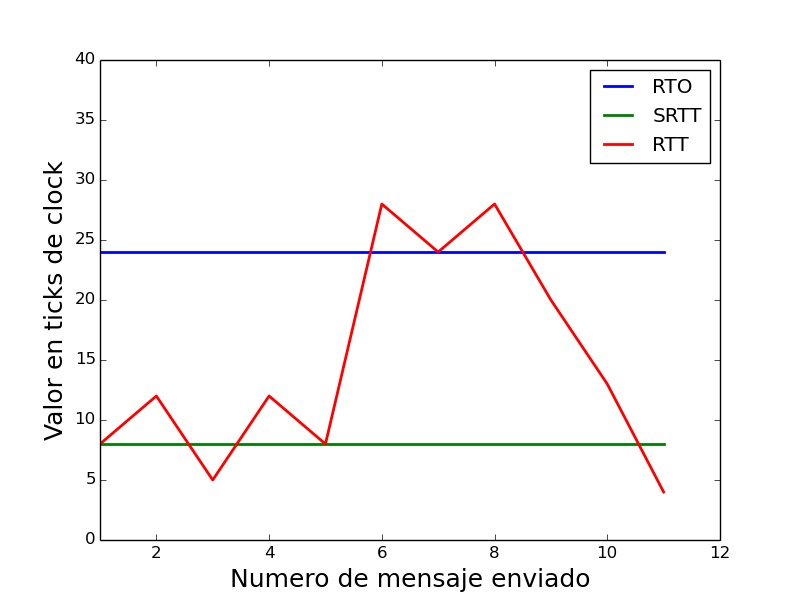
\includegraphics[scale=0.32]{imagenes/ALPHA_0_BETA_0.jpg}
      \caption{RTO, SRTT y RTT para ALPHA=0 y BETA=0}
  \end{center}
\end{figure}

Tal como puede esperarse, tomando $\alpha=0$, $\beta=0$ los cálculos ignoran por completo los nuevos
valores de RTT y consideran únicamente los valores de SRTT anteriores. En este caso, el valor constante
inicial.

\begin{figure}[H]
  \begin{center}
      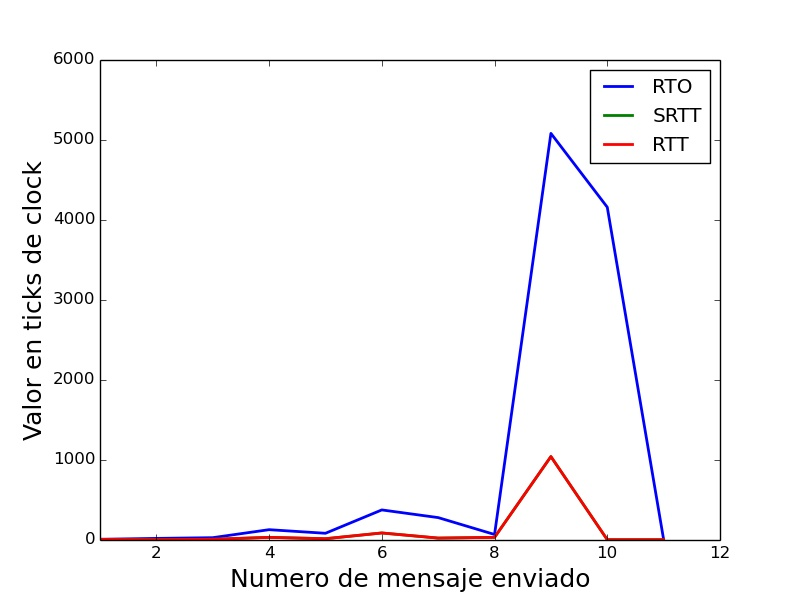
\includegraphics[scale=0.32]{imagenes/ALPHA_1_BETA_1.jpg}
      \caption{RTO, SRTT y RTT para ALPHA=1 y BETA=1}
  \end{center}
\end{figure}

Este experimento es completamente opuesto al anterior. Tomando ambas variables como 1, los cálculos
ignoran los valores anteriores (tanto de variación de RTT (RTTVAR) somo de SRTT), y modifican
los resultados únicamente en función de la última muestra de RTT obtenida. El resultado es un gráfico
en donde el RTO coincide exactamente con el SRTT, y ambos responden excesivamente a cualquier fluctuación
que se produzca en el valor del RTT.


\begin{figure}[H]
  \begin{center}
      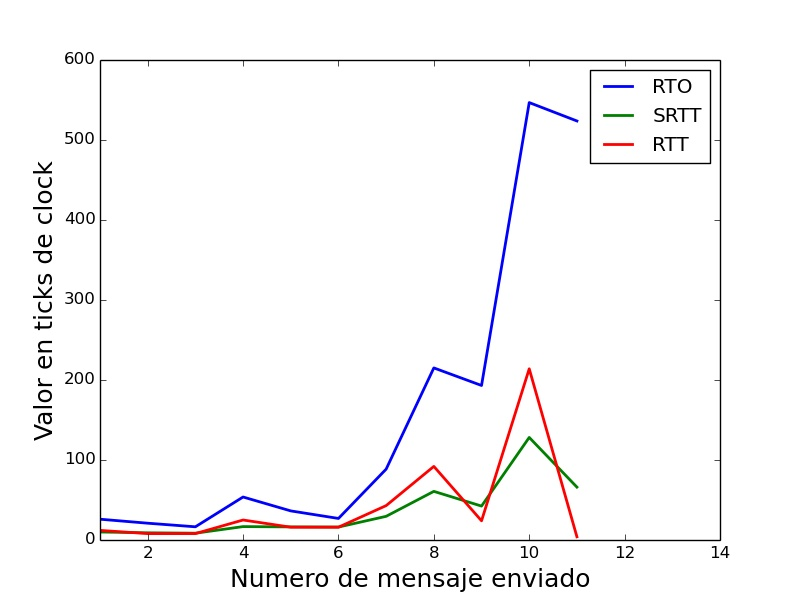
\includegraphics[scale=0.32]{imagenes/ALPHA_050_BETA_050.jpg}
      \caption{RTO, SRTT y RTT para ALPHA=0.5 y BETA=0.5}
  \end{center}
\end{figure}

Una de las primeras ideas que tuvimos fue
ponderar de igual manera los valores anteriores con los nuevos, al tomar ambas variables con valor
0.5. Esto debería generar valores cercanos a los de lasmuestras anteriores, pero que sean capaces
de responder a cambios significativos y permanentes del valor de RTT. En otras palabras, que alcancen
un equilibrio entre ambas propuestas. Sin embargo, el comportamiento no fue el esperado.
El resultado es una serie de cálculos demasiado sensibles a las fluctuaciones temporales que responden
excesivamente a estos cambios.

\begin{figure}[H]
  \begin{center}
      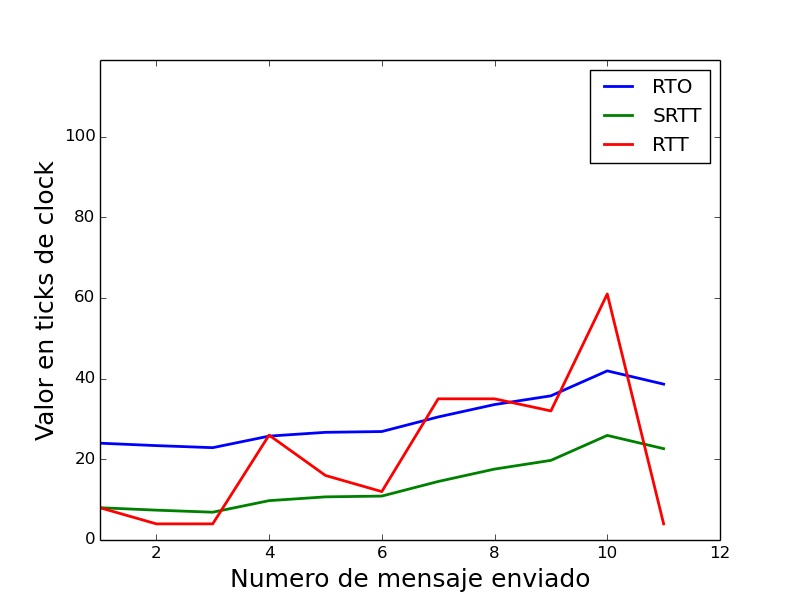
\includegraphics[scale=0.32]{imagenes/ALPHA_015_BETA_0.jpg}
      \caption{RTO, SRTT y RTT para ALPHA=0.15 y BETA=0}
  \end{center}
\end{figure}

Habiendo convalidado las hipótesis anteriores nos parece razonable fijar el valor de $\alpha$ en 0.15 (
cercano al propuesto por el RFC 6298). Las conexiones en las distintas redes por lo general permanecen
estables la mayor parte del tiempo (con lo cual la probabilidad de que el rtt permanezca inalterable
es alta), y los cambios considerables en el valor del round-trip-time son más esporádicos. De cualquier
manera, dejamos una ventana considerable para que cualquier cambio significativo en el RTT impacte
en los cálculos del SRTT. Es notorio el hecho de que el RTO aproxima bastante bien la curva del RTT, pero
lo hace de forma suave, a diferencia de esta última.

\begin{figure}[H]
  \begin{center}
      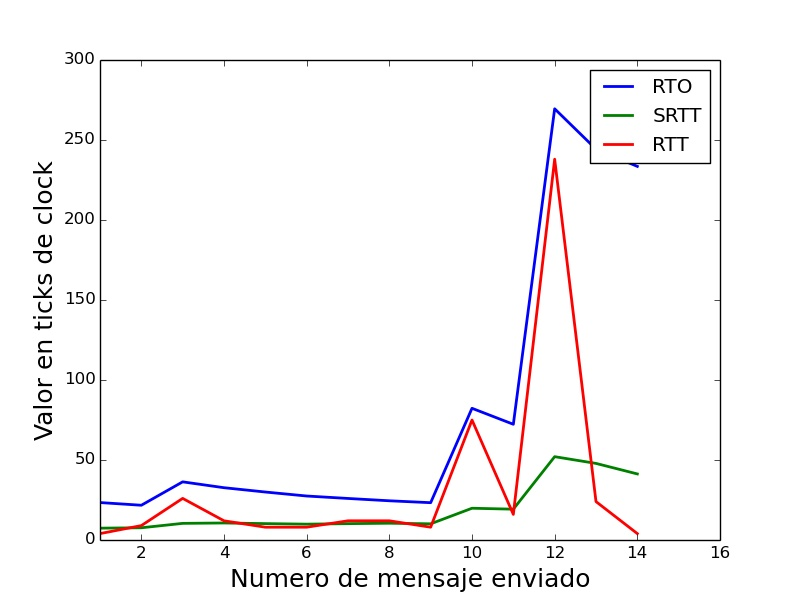
\includegraphics[scale=0.32]{imagenes/ALPHA_015_BETA_020.jpg}
      \caption{RTO, SRTT y RTT para ALPHA=0.15 y BETA=0.20}
  \end{center}
\end{figure}

Estos valores hacen que el algoritmo calcule valores mucho más cercanos a los RTT reales, a diferencia
del anterior. Ambos cambios repentinos en los valores del RTT (vistos en el gráfico como picos) son
correctamente advertidos por el cálculo del RTO. Esto se debe a que el valor de BETA cambia de 0 a
0.2, con lo cual se le agrega un poco más de sensibilidad a los cambios en el valor de los RTT's.

\begin{figure}[H]
  \begin{center}
      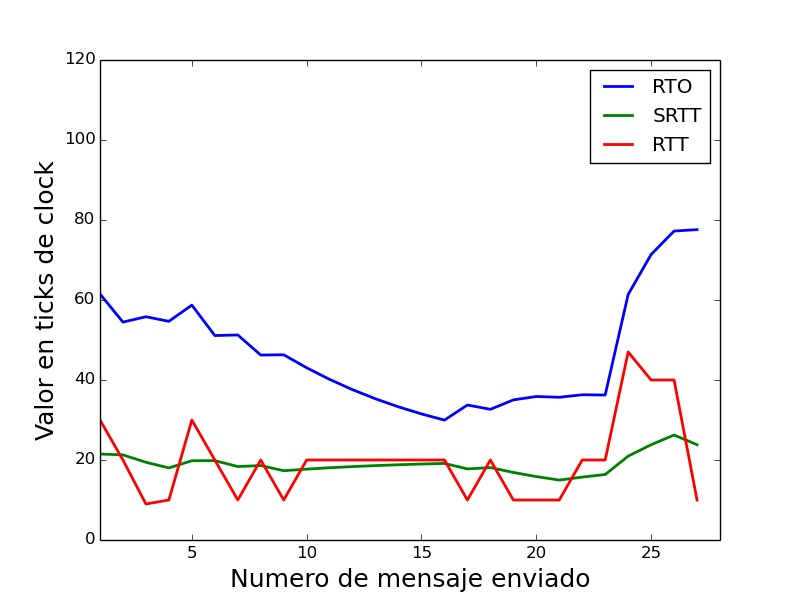
\includegraphics[scale=0.32]{imagenes/OPTIMOS_MARCO_REAL.jpg}
      \caption{RTO, SRTT y RTT para ALPHA=0.15 y BETA=0.20 en un marco real}
  \end{center}
\end{figure}

Finalmente agregamos un experimento en donde observamos el comportamiento de las actualizaciones en
un marco más real. Establecemos el valor de probabilidad de pérdida en 0.05 y el valor del delay en
10 ms.
Los valores de las variables seleccionadas se comportan realmente bien. Por un lado responden de manera
sensible a los cambios en el valor de los RTT. En suma, cuando no se
producen este tipo de cambios (situaciones hipotéticas en donde no se caigan nodos dentro de la red, o
la misma no se encuentre congestionada), el algoritmo pondera los valores anteriores y de a poco
converge al valor del RTT real.

Por estos motivos, decidimos seleccionar los valores de $\alpha=0.15$ y $\beta=0.20$.









\subsection{Resultados}

    \subsubsection{Valor de RTO variando $\alpha$ y $\beta$}
        Los resultados de medir el \rto{} para un valor fijo de 
        \textit{25 ticks} y probabilidad de perdida cero luego de 
        enviar 200 paquetes se pueden ver en la \emph{Figura 1}.
        
    \subsubsection{Perdida de paquetes variando $\alpha$ y $\beta$}
        Para estudiar la perdida de paquetes se fij\'o el valor de 
        de \rto{} en \textit{25 ticks} y no se simularon p\'erdidas.
        Sin embargo en varios casos hubo retransmisiones, la 
        \textit{Figura 2} muestra el resultado para el env\'io de 150
        paquetes mientras que la \textit{Figura 3} lo muestra para 300.
        
    \begin{figure}[H]
	    \center
	    \begin{subfigure}{0.32\textwidth}
		    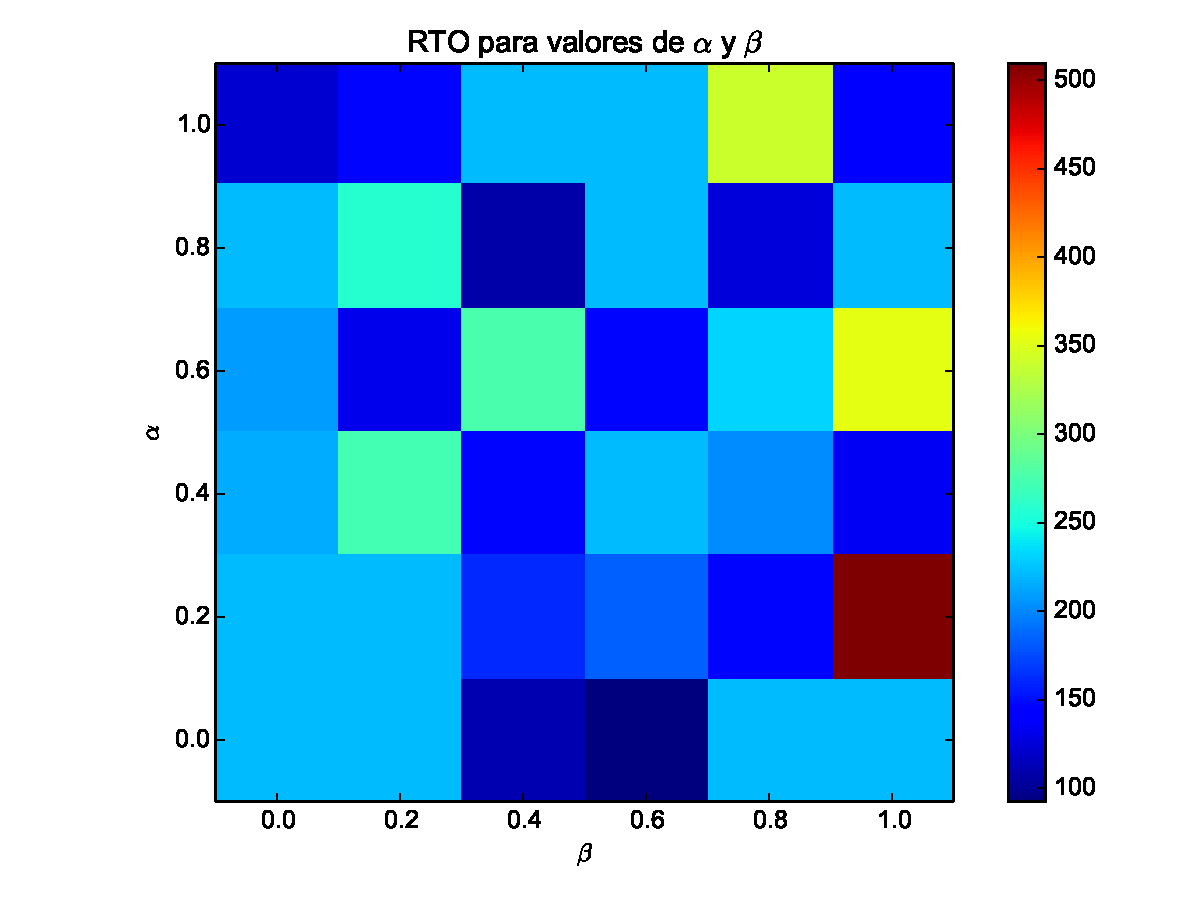
\includegraphics[width=1.0\textwidth]{imagenes/guille/rto_vs_alphaBeta.pdf}
		    \caption{Figura 1}
	    \end{subfigure}
	    ~
	    \begin{subfigure}{0.32\textwidth}
		    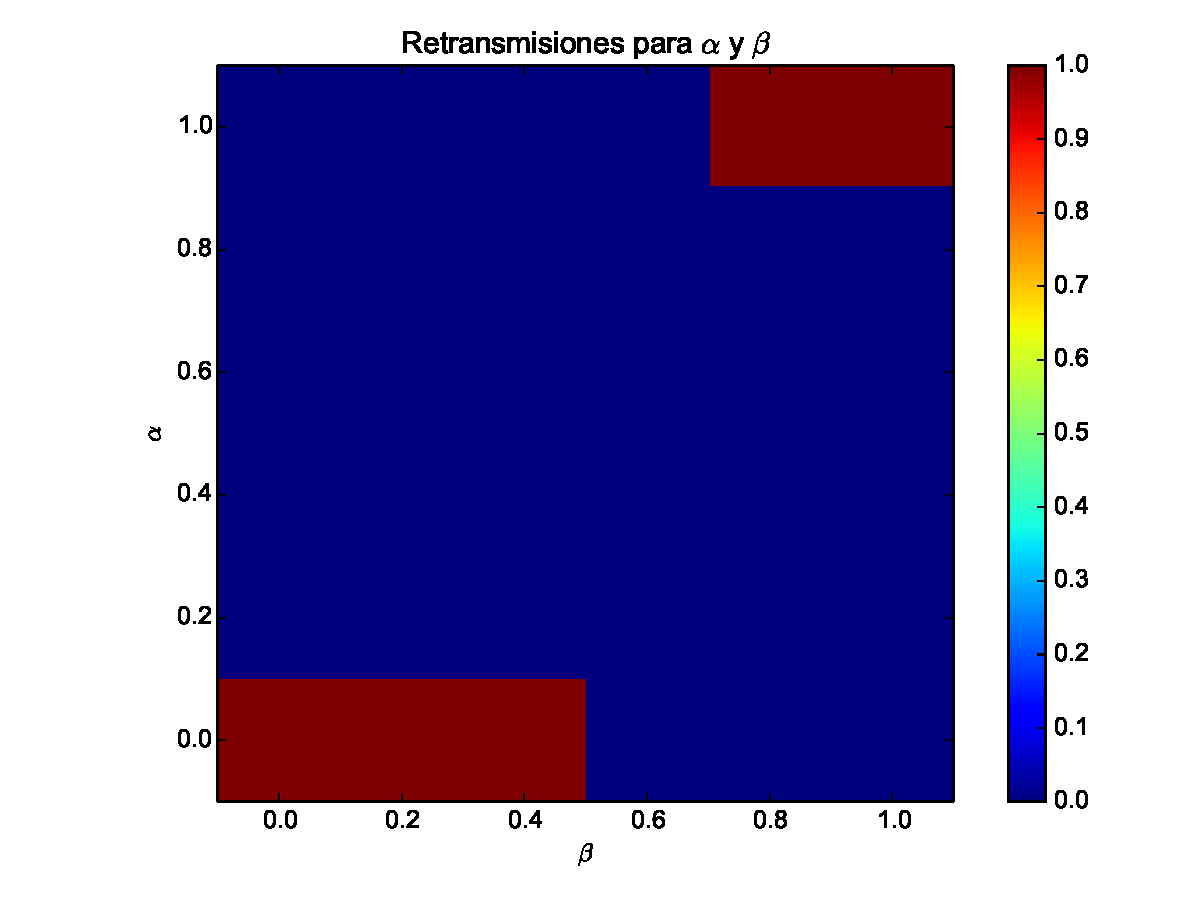
\includegraphics[width=1.0\textwidth]{imagenes/guille/retransmisiones_150.pdf}
		    \caption{Figura 2}
	    \end{subfigure}
	    ~
	    \begin{subfigure}{0.32\textwidth}
		    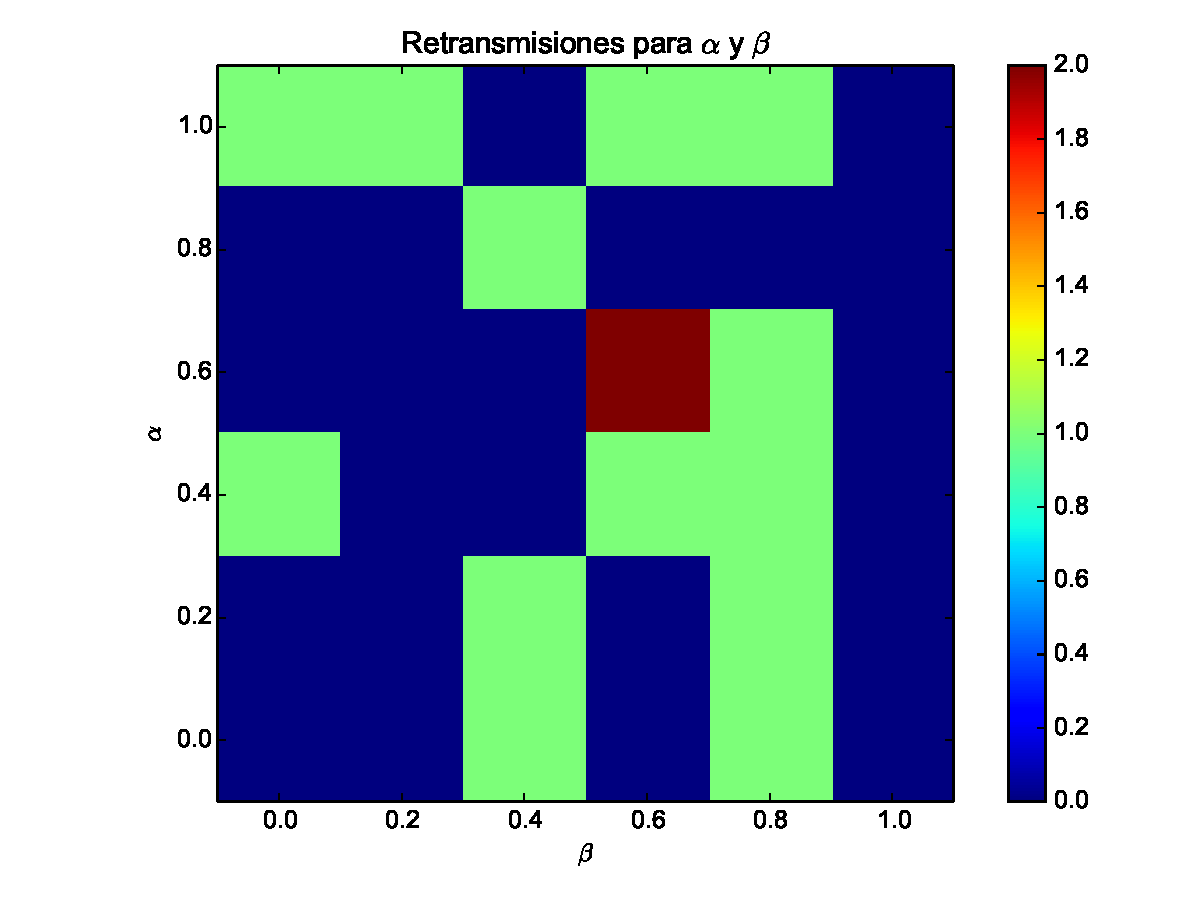
\includegraphics[width=1.0\textwidth]{imagenes/guille/retransmisiones_300.pdf}
		    \caption{Figura 3}
	    \end{subfigure}
	
    \end{figure}    


    \subsubsection{Valor de RTO cuando la red se congestiona sin perdida}
        Para este configuramos el cliente para que env\'ie 300 paquetes al
        servidor, pero luego de enviarse 150 paquetes, el delay de la red
        se duplicara o cuadruplicara. 
        
        El \emph{Escenario 1} muestra el resultado en una red con
        par\'aemtros: $\alpha={{1}\over{2}}$, $\beta={{1}\over{4}}$
        cuando no se congestiona, cuando la congesti\'on causa el doble de
        delay, y cuando causa el cuadruple.
  
        \begin{figure}[H]
            \center
	        
		    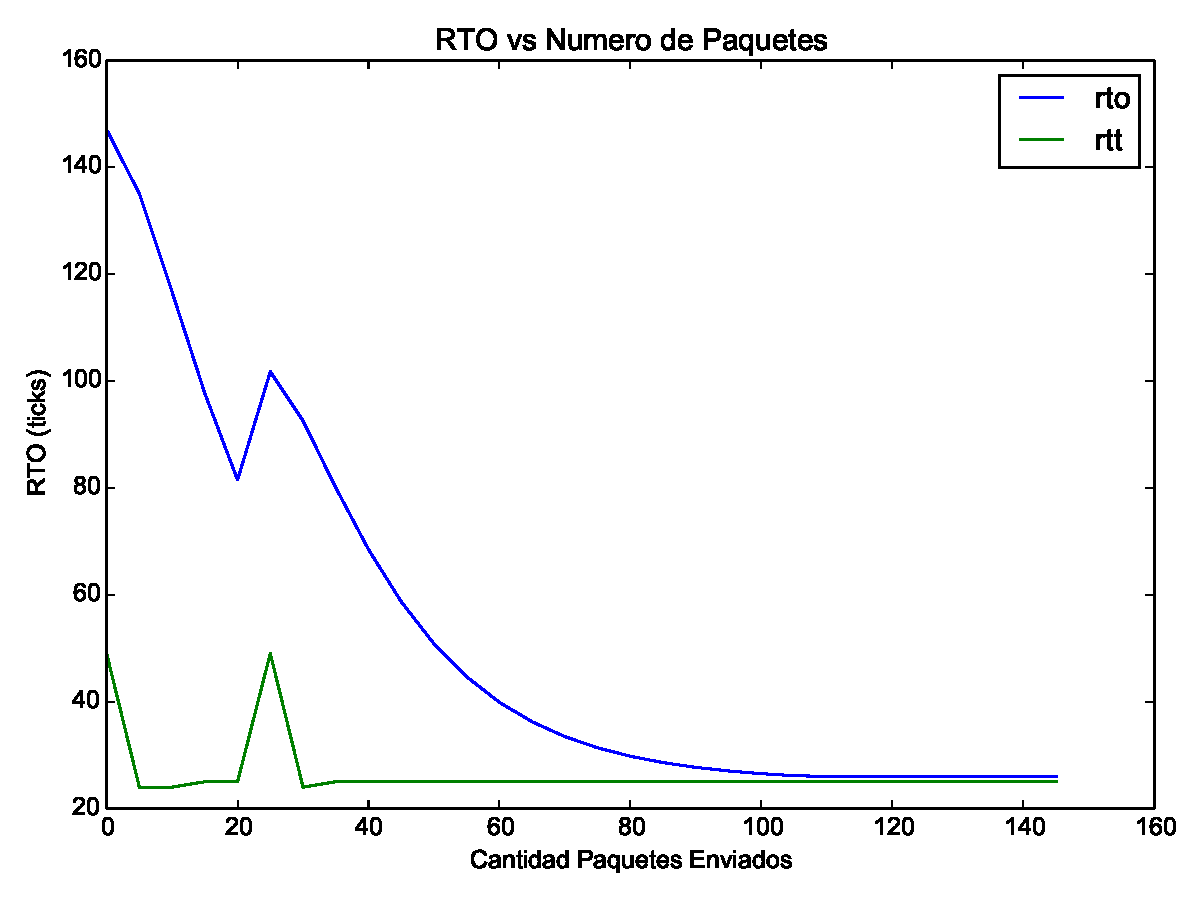
\includegraphics[width=0.32\textwidth]{imagenes/guille/rtt_vs_n_2_4.pdf}
		    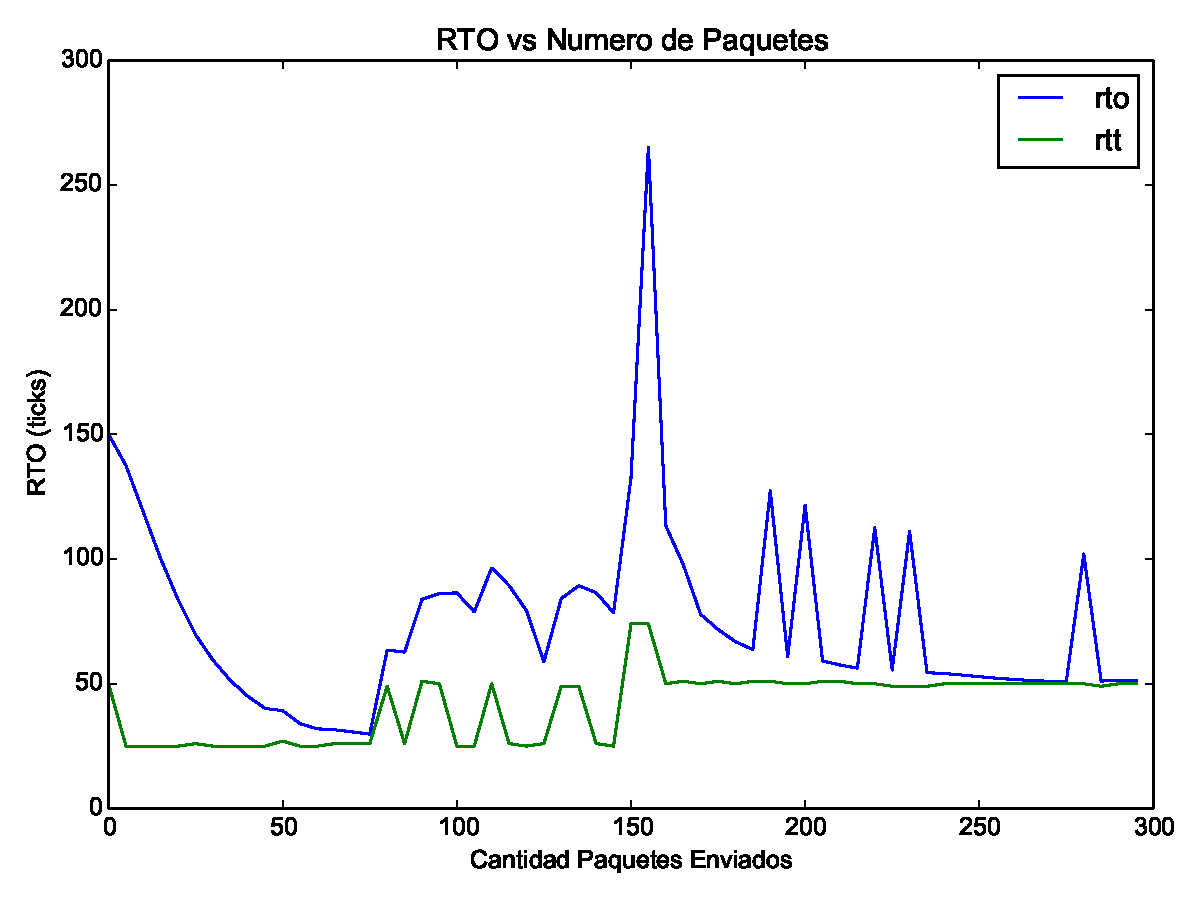
\includegraphics[width=0.32\textwidth]{imagenes/guille/congestion_50_2_4.pdf}
		    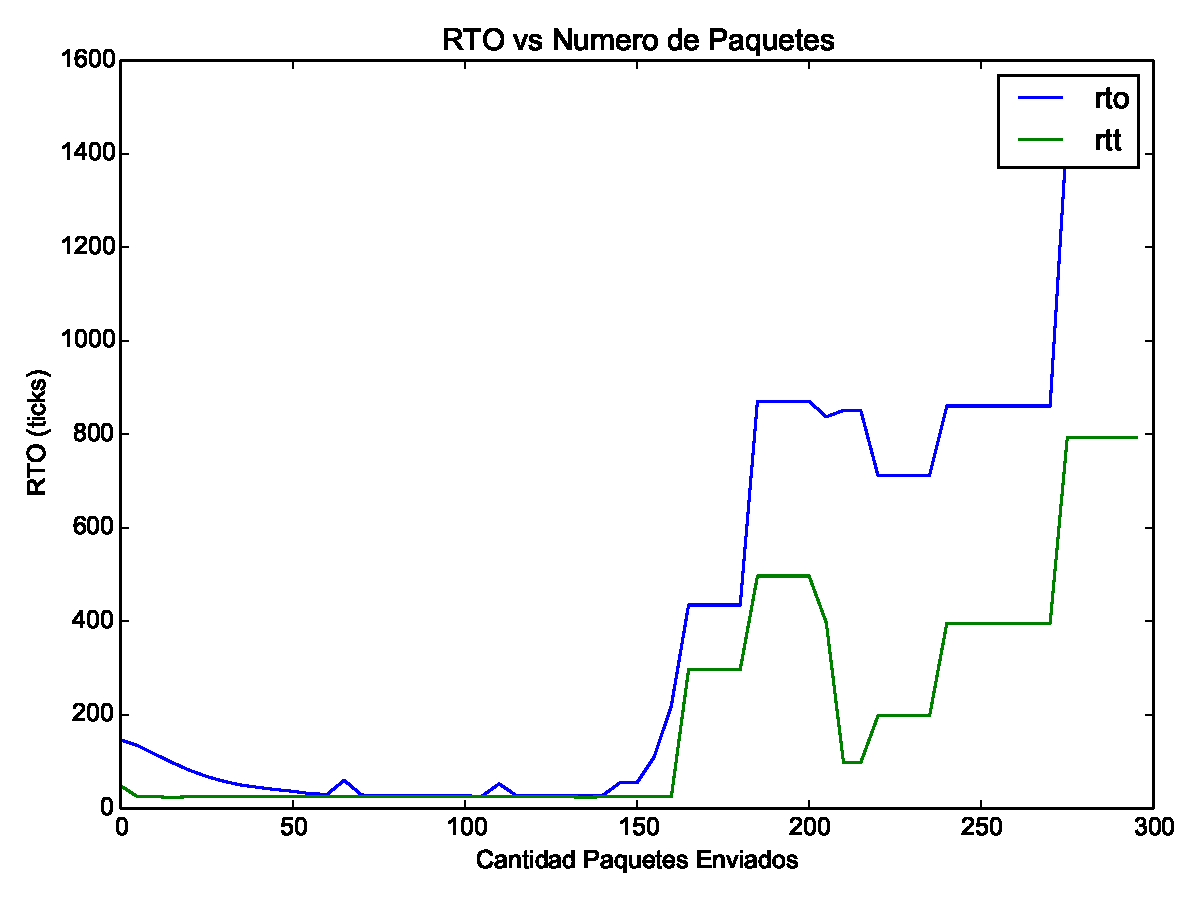
\includegraphics[width=0.32\textwidth]{imagenes/guille/congestion_100_2_4.pdf}

            \caption{Escenario 1}
	
        \end{figure}          
  
        El \emph{Escenario 2} muestra el resultado en una red con
        par\'aemtros: $\alpha={{1}\over{8}}$, $\beta={{1}\over{2}}$ 
        cuando no se congestiona, cuando la congesti\'on causa el doble de
        delay, y cuando causa el cuadruple.

        \begin{figure}[H]
            \center
	        
		    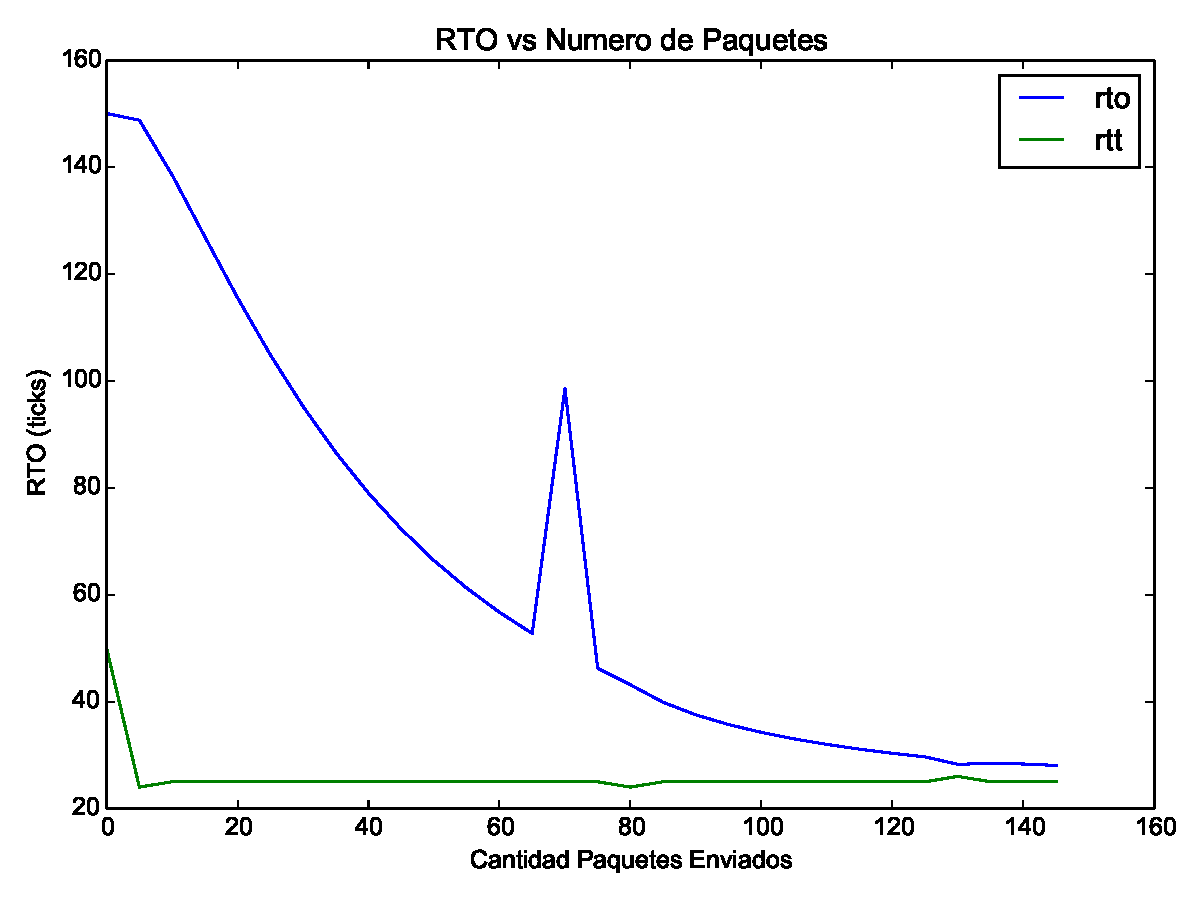
\includegraphics[width=0.32\textwidth]{imagenes/guille/rtt_vs_n_8_2.pdf}
		    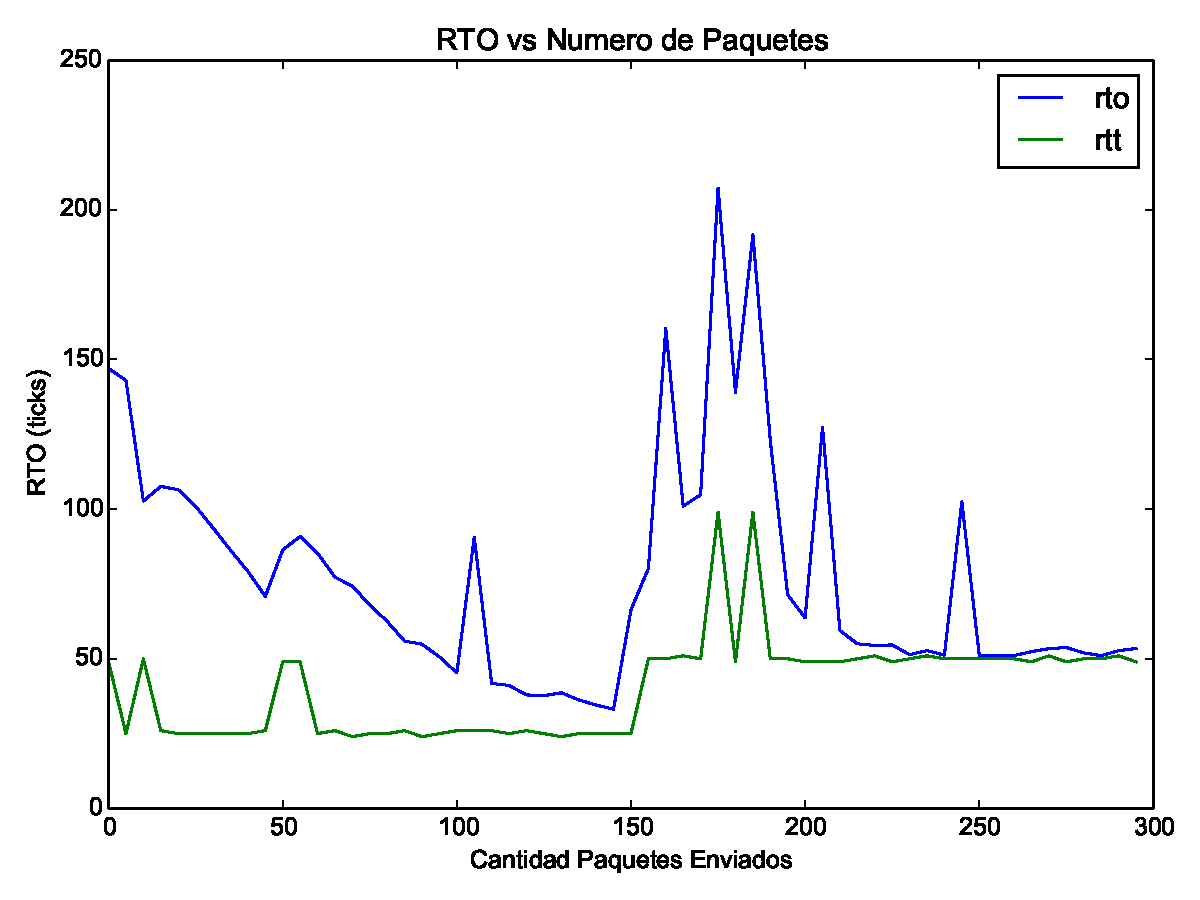
\includegraphics[width=0.32\textwidth]{imagenes/guille/congestion_50_8_2.pdf}
		    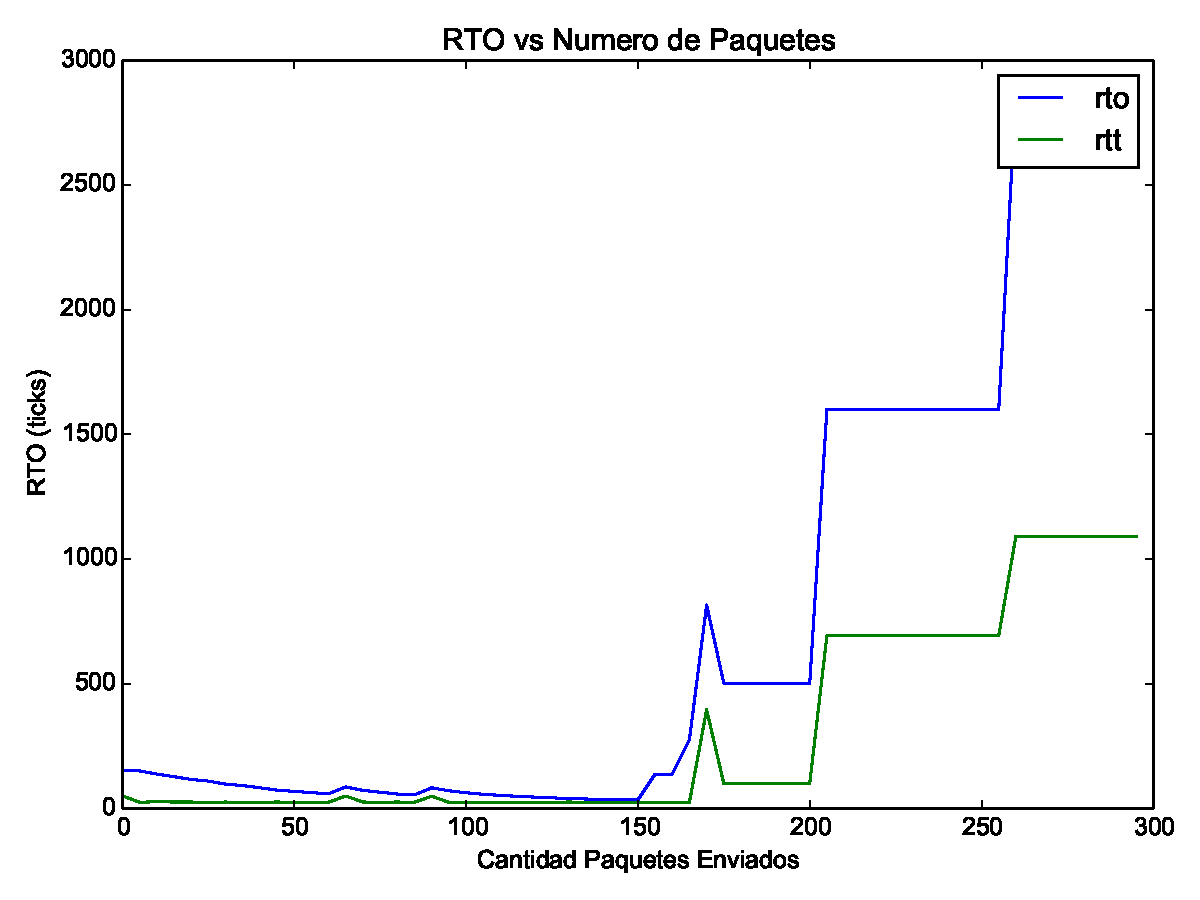
\includegraphics[width=0.32\textwidth]{imagenes/guille/congestion_100_8_2.pdf}

            \caption{Escenario 1}
	
        \end{figure}          

        En ambos casos sucedi\'o que al duplicar el valor del delay el 
        mensaje n\'umero 101 debi\'o ser retransmitido. A su vez, cuando 
        se cuadruplic\'o el valor de la red, el mensaje n\'umero 101 debi\'o
        ser retransmitido dos veces. 
        Tambi\'en se puede notar que en ambos casos luego de cuadruplicarse
        el delay no se logr\'o volver a un \rto{} cercano a el \rtt{} real.



%\section{Conclusiones}

Todos los experimentos demostraron lo susceptible que es la medici\'on de
RTO a los par\'ametros de la red, as\'i como tambi\'en a los par\'ametros
utilizados para estimarlo. 

Primero vimos que cambiar los valores de $\alpha$ y $\beta$ modifican
significativamente el valor estimado de \rto{}, al experimentar con valores
muy peque\~nos, los cálculos no se adaptan de forma realista a las
variaciones en los valores de RTT reales. Por el contrario, al tomar
valores muy altos los mismos se ven demasiado influenciados por
fluctuaciones temporales, dando como resultado valores demasiado altos o
demasiado peque\~nos en comparación con el RTT real. 

Luego vimos como los valores de $\alpha$ y $\beta$ modifican la cantidad
de retransmisiones, cabe destacar que las \textit{Figuras 5 y 6} son parte
de un experimento en el cual no se simul\'o perdida de paquetes, sin embargo
, hubo retransmisiones. Esto se debe a que cuando el \rto{} se acerca al 
\rtt{} estimado es muy sensible a cambios internos de la pc, recordemos que
los procesos de cliente y servidor est\'an funcionando dentro de un sistema
operativo hogareño. 

Por \'ultimo, vimos como el c\'alculo del \rto{} afecta a la transmisi\'on
total de una conexi\'on. Podemos ver que entre el primer resultado hay casi
dos segundos de diferencia, teniendo en cuenta que el tiempo para enviar un 
mensaje entre ambos nodos es menor a 0.1 seg, podemos ver que la diferencia
de performance es notable.

Para concluir queremos agregar que el valor que mejor funcion\'o en los 
experimentos fue el propuesto por el RFC, consiguiendo aproximarnos con $\alpha=0.15$ y $\beta=0.2$. 


\section{Referencias}
\begin{itemize}
	\item \textbf{Computer Networks: A Systems Approach}, \textit{Larry L. Peterson and Bruce S. Davie.}
	\item \textbf{Computer Networks}, \textit{Andrew S. Tanenbaum}
%	\item \textbf{http://submarinecablemap.com/}
%	\item \textbf{Special-Purpose IP Address Registries} (RFC 6890), \textit{Internet Engineering Task Force (IETF)}
%	\item \textbf{An Ethernet Address Resolution Protocol or Converting Network Protocol Addresses to 48.bit Ethernet Address for Transmission on Ethernet Hardware} (RFC 826), \textit{David C. Plummer}
\end{itemize}

\end{document}
